\documentclass[10pt]{article}
\usepackage[margin=1in, paperwidth=8.5in, paperheight=11in]{geometry}
\usepackage{ifpdf,amsmath, amssymb, comment, color, graphicx, stmaryrd,setspace,enumitem,tikz, fancyhdr, wrapfig, textcomp, mathptmx, siunitx}
\usepackage{tikz}
\usetikzlibrary{trees}

\setlength{\headheight}{14.5pt}
\newcommand{\Q}{\mathbb{Q}}
\newcommand{\R}{\mathbb{R}}
\newcommand{\Z}{\mathbb{Z}}
\newcommand{\vu}{\mathbf{u}}
\newcommand{\vv}{\mathbf{v}}
\newcommand{\vw}{\mathbf{w}}
\newcommand{\vi}{\mathbf{i}}
\newcommand{\vj}{\mathbf{j}}
\newcommand{\vk}{\mathbf{k}}
\newcommand{\vn}{\mathbf{n}}
\newcommand{\vr}{\mathbf{r}}
\newcommand{\va}{\mathbf{a}}
\newcommand{\vF}{\mathbf{F}}
\newcommand{\vL}{\mathbf{L}}
\newcommand{\vT}{\mathbf{T}}
\newcommand{\vN}{\mathbf{N}}
\newcommand{\proj}{\operatorname{proj}}
\newcommand{\orth}{\operatorname{orth}}
\newcommand\dotp[1][.5]{\,\mathbin{\vcenter{\hbox{\scalebox{#1}{$\bullet$}}}}\,}

% Solution text is in red. If you want the solutions to show, remove the \iffalse from the definition of the \red command.
%\newcommand{\red}[1]{ %\iffalse
%	\textcolor{red}{#1} }%\fi}

\newenvironment{red}{\color{red}}{\ignorespacesafterend}
\newcommand{\blue}[1]{\textcolor{blue}{#1}}
\newcommand{\green}[1]{\textcolor{green}{#1}}
\renewcommand{\section}[1]{\begin{center} \textbf{#1} \\\end{center}}
%
\hyphenpenalty=5000
\setlength{\parindent}{0in}
%\oddsidemargin=-.25in
\allowdisplaybreaks
\pagestyle{fancy}
\renewcommand{\headrulewidth}{0pt}
\lhead{MATH 203}
\rhead{Fall 2019}
%\lfoot{\copyright\ CLEAR Calculus 2010}
\cfoot{}

\begin{document}
%


%\onehalfspacing
\allowdisplaybreaks
%##################################################################
\section{PS\#7 -- Linearization; chain rule - \red{Answer key} }

\begin{enumerate}[leftmargin=0pt]
    
    \item (Arc length problem to apply to Exam 1) 
    \begin{itemize}
        \item Go to CalcPlot3D and pick a space curve from the "Examples" menu. Choose something that has a nonzero z component, so that it actually is a space curve rather than just a plane curve.
        
        \begin{red}
        I chose Viviani's curve (which, interestingly, is the intersection between a sphere and a cylinder that's tangent to the sphere and goes through the center of the sphere).
        \end{red}
        \item Write down the integral that will allow you to calculate the arc length of the space curve you've chosen. What should your bounds of integration be?
        
        \begin{red}
        The integrand is $|\vr'(t)|$:
        \begin{align*}
            \vr(t) &= \left\langle 1 + \cos t, \sin t, 2 \sin \tfrac{t}{2} \right\rangle \\
            \vr'(t) &= \left\langle -\sin t, \cos t, \cos \tfrac{t}{2} \right\rangle \\
            |\vr'(t)| &= \sqrt{ 
            (-\sin t)^2 + (\cos t)^2 + \left(\cos \tfrac{t}{2}\right)^2
            }\\
            &= \sqrt{\sin^2 t + \cos^2 t + \cos^2\left(\tfrac{t}{2}\right)} \\
            &= \sqrt{1 + \cos^2\left(\tfrac{t}{2}\right)}
        \end{align*}
        (I imagine I could use some trig identities to simplify this further, but I don't ever remember any trig identities besides the Pythagorean identity, lol.)
        
        My bounds of integration should be from $-2\pi$ to $2\pi$, based on the bounds that are programmed into CalcPlot3D. As I look at the ``trace'' arrows moving around the curve, this does indeed appear to produce one full trip around the curve.
        
        So, my integral should be:
        \[ \int_{-2\pi}^{2\pi} \sqrt{1 + \cos^2\left(\tfrac{t}{2}\right)} \, dt \]
        \end{red}
        \item Your integrand probably does not have an antiderivative. That means you can't use the fundamental theorem of calculus to compute your definite integral. Darn! Use computing technology (W$|$A?) to find a numerical approximation to the value of your definite integral. 
        
        \begin{red}
        Fun fact: you can type LaTeX directly into Wolfram$|$Alpha and it will interpret it correctly. Here's my result:
        \begin{center}
            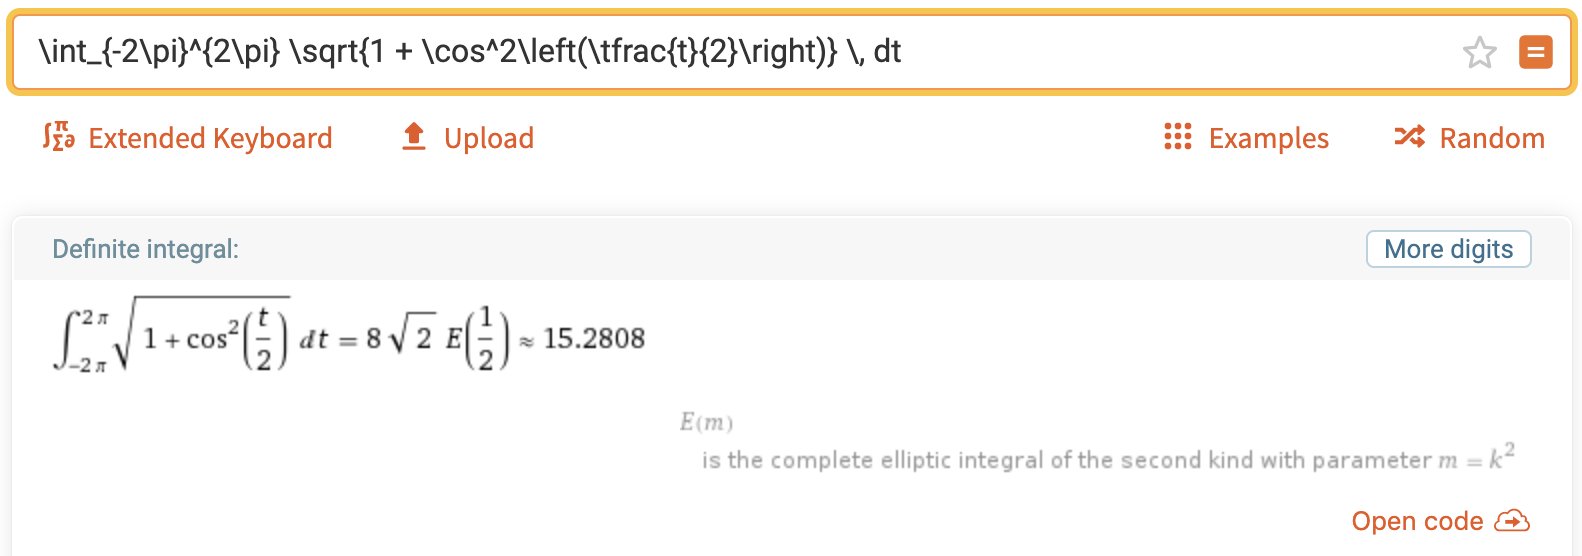
\includegraphics[width=0.75\textwidth]{wa-arc-length.png}
        \end{center}
        This whole business about ``the complete elliptic integral of the second kind'' is W$|$A telling you that there's no elementary antiderivative of this particular integrand. Fortunately, it's smart enough to compute a pretty good numerical approximation, 15.2808.
        \end{red}
        \item Looking at your graph on CalcPlot3D, does your numerical value seem about right? (If not, perhaps you set up your integral wrong?) Write a couple of sentences explaining why your value looks plausible.
        
        \begin{red}
        Yeah, I guess I buy this. I think you could reasonably approximate this curve by gluing a couple of circles with radius $\sqrt{2}$ together, and each one of those is going to have circumference $2\cdot\pi\cdot\sqrt{2} \approx 2 \cdot 3 \cdot 1.5 = 9$. So getting something close to 18 is pretty good, I guess.
        \end{red}
    \end{itemize}
    \pagebreak
    
    \item (Your favorite part of \#13 or \#14 in AC Multi 2.4)
    \begin{itemize}
        \item[13a.] Find the linearization $L(x,y)$ for the function $f$ defined by $f(x,y) = \cos(x)(2e^{2y}+e^{-2y})$ at the point $(x_0, y_0) = (0, 0)$. Hence use the linearization to estimate the value of $f(0.1, 0.2)$. Compare your estimate to the actual value of $f(0.1, 0.2)$.
        
        \begin{red}
        First let's compute all the values we'll need:
        \begin{align*}
            f(0, 0) &= \cos(0)(2e^{2\cdot 0}+e^{-2\cdot 0}) = 3 \\
            f_x(x,y) &= -\sin(x)(2e^{2y}+e^{-2y}) \\
            f_x(0,0) &= -\sin(0)(2e^{2\cdot 0}+e^{-2\cdot 0}) = 0 \\
            f_y(x, y) &= \cos(x)(4e^{2y}-2e^{-2y}) \\
            f_y(0, 0) &= \cos(0)(4e^{2\cdot 0}-2e^{-2\cdot 0}) = 2
        \end{align*}
        Cool, so the linearization $L(x, y) = 3 + 0\cdot(x-0) + 2\cdot(y-0) = 3 + 2y.$
        
        So, $f(0.1, 0.2) \approx L(0.1, 0.2) = 3 + 2\cdot 0.2 = 3.4$. 
        
        The actual value is $f(0.1, 0.2) = 3.63571$, per W$|$A. 3.4 is pretty dang close!
        \end{red}
        
        \item[13b.] The Heat Index, $I$ (measured in apparent degrees F), is a function of the actual temperature $T$ outside (in degrees F) and the relative humidity $H$ (measured as a percentage). A portion of the table which gives values for this function, $I = I(T, H)$, is provided below:
        \[
        \begin{array}{ccccc}\hline T \downarrow \backslash H \rightarrow & {70} & {75} & {80} & {85} \\ \hline 90 & {106} & {109} & {112} & {115} \\ \hline 92 & {112} & {115} & {119} & {123} \\ \hline 94 & {118} & {122} & {127} & {132} \\ \hline 96 & {125} & {130} & {135} & {141} \\ \hline\end{array}
        \]
        Suppose you are given that $I_T(94,75) = 3.75$ and $I_H(94, 75) = 0.9$. Use this given information and one other value from the table to estimate the value of $I(93.1, 77)$ using the linearization at $(94, 75)$. Using proper terminology and notation, explain your work and thinking.
        
        \begin{red}
        Okay, so we'll also need a starting value. From the table, $I(94,75) = 122$. (Yikes!)
        
        Now we have enough information to write down the linearization:
        
        \begin{align*}
            L(T, H) &= I(94, 75) + I_T(94, 75)(T - 94) + I_H(94, 75) (H - 75) \\
            &= 122 + 3.75(T - 94) + 0.9 (H - 75)
            \intertext{I could simplify this, but I think this will actually be easier to work with as is:}
            I(93.1, 77) \approx L(93.1, 77) &=
            122 + 3.75(93.1 - 94) + 0.9 (77-75) \\
            &= 122 + 3.75 (-0.9) + 0.9 (2) \\
            &= 122 + (-3.375) + 1.8 = 122 -1.575 \\
            &= 120.425
        \end{align*}
        What I really like about this is it shows the contribution of each change from our starting point to the overall heat index. Dropping the temperature to 93.1$^\circ$, a decrease of $0.9^\circ$, caused the heat index to drop by 3.375$^\circ$, and increasing the humidity to 77\%, an increase of $2\%$, caused the heat index to go up by 1.8$^\circ$, for a total change of -1.575$^\circ$. So we end up dropping 1.575$^\circ$ from $122^\circ$ to land at 120.425$^\circ$.
        \end{red}
        
        \item[13c.] Just as we can find a local linearization for a differentiable function of two variables, we can do so for functions of three or more variables. By extending the concept of the local linearization from two to three variables, find the linearization of the function $h(x,y,z) = e^{2x}(y+z^2)$ at the point $(x_0,y_0,z_0) = (0, 1, -2)$. Then, use linearization to estimate the value of $h(-0.1, 0.9, -1.8)$.
        
        \begin{red}
        First let's compute all the values we'll need:
        \begin{align*}
            h(0, 1, -2) &= e^{2\cdot 0}(1 + (-2)^2) = 5 \\
            h_x(x,y,z) &= 2 e^{2x}(y + z^2) \\
            h_x(0, 1, -2) & =2 e^{2\cdot 0}(1 + (-2)^2) = 10 \\
            h_y(x,y,z) &= e^{2x}(1) \\
            h_y(0, 1, -2) &= e^{2\cdot 0} = 1 \\
            h_z(x,y,z) &= e^{2x}(2z) \\
            h_z(0, 1, -2) &= e^{2\cdot 0} (2\cdot(-2)) = -4 \\
            \intertext{Putting this all together,}
            L(x,y,z) &= 5 + 10(x-0) + 1(y-1) + (-4)(z + 2) \\
            h(-0.1, 0.9, -1.8) \approx 
            L(-0.1, 0.9, -1.8) &= 5 + 10(-0.1 - 0) + 1(0.9-1)+(-4)(-1.8 + 2) \\
            &= 5  -1 -0.1 -0.8 = 3.1
        \end{align*}
        Just for fun, the actual value of $h(-0.1, 0.9, -1.8)$ is 3.38955. Pretty decent approximation!
        \end{red}
        
        \item[14a.] Let $f$ represent the vertical displacement in centimeters from the rest position of a string (like a guitar string) as a function of the distance $x$ in centimeters from the fixed left end of the string and $y$ the time in seconds after the string has been plucked. A simple model for $f$ could be \[f(x, y) = \cos(x)\sin(2y).\]
        Use the differential to approximate how much more this vibrating string is vertically displaced from its position at $(a,b) = \left(\tfrac{\pi}{4}, \tfrac{\pi}{3}\right)$ if we decrease $a$ by $0.01$ cm and increase the time by 0.1 seconds. Compare to the value of $f$ at the point $\left(\tfrac{\pi}{4}-0.01, \tfrac{\pi}{3}+0.1\right)$.
        
        \begin{red}
        First let's compute the partial derivatives:
        \begin{align*}
            f_x(x,y) &= -\sin(x)\sin(2y) \\
            f_x\left(\frac{\pi}{4}, \frac{\pi}{3}\right)
            &= -\sin\left(\frac{\pi}{4}\right) \sin\left(2\cdot\frac{\pi}{3}\right) = -\frac{\sqrt{6}}{4} \approx -0.6124 \\
            f_y(x,y) &= 2\cos(x)\cos(2y) \\
            f_y\left(\frac{\pi}{4}, \frac{\pi}{3}\right)
            &=2\cos\left(\frac{\pi}{4}\right)\cos\left(2\cdot\frac{\pi}{3}\right) = -\frac{\sqrt{2}}{2} \approx -0.7071 \\
            \intertext{Now we can write down the differential:}
            df &= f_x\left(\frac{\pi}{4}, \frac{\pi}{3}\right) dx + f_y\left(\frac{\pi}{4}, \frac{\pi}{3}\right) dy \\
            &= -0.6124\, dx - 0.7071\, dy \\
            \intertext{We're given that $dx=-0.01$ and $dy=0.1$, so}
            df &= -0.6124\cdot(-0.01) - 0.7071\cdot 0.1 = -0.064586.
        \end{align*}
        The value of $f$ at the point $\left(\tfrac{\pi}{4}-0.01, \tfrac{\pi}{3}+0.1\right)$ is about 0.5351982. The value of $f$ at the point $\left(\tfrac{\pi}{4}, \tfrac{\pi}{3}\right)$ is about 0.6123724. That makes for an actual change $\Delta f$ of $ 0.5351982 - 0.6123724 = -0.0771742,$ which is pretty close to the approximate change $df$ we calculated.
        \end{red}
        \pagebreak
        
        \item[14b.] Resistors used in electrical circuits have colored bands painted on them to indicate the amount of resistance and the possible error in the resistance. When three resistors, whose resistances are $R_1$, $R_2$, and $R_3$, are connected in parallel, the total resistance $R$ is given by \[\frac1R = \frac1{R_1} + \frac1{R_2} + \frac1{R_3}.\]
        Suppose that the resistances are $R_1 = 25\Omega$, $R_2 = 40\Omega$, and $R_3 = 50\Omega$. Find the total resistance $R$. If you know each of $R_1$, $R_2$, and $R_3$ with a possible error of $0.5\%$, estimate the maximum error in your calculation of $R$.
        
        \begin{red}
        So, first of all, the total resistance:
        \begin{align*}
            \frac1R &= \frac1{R_1} + \frac1{R_2} + \frac1{R_3} \\
            &= \frac{1}{25} + \frac{1}{40} + \frac{1}{50} = \frac{17}{200} \\
            R &= \frac{200}{17} \approx 11.7647.
        \end{align*}
        We now need to figure out each of the differentials, which should be $0.5\%$ of each resistance value. So, $dR_1 = 0.005\cdot 25 = 0.125$, $dR_2 = 0.005\cdot 40 = 0.2$, and $dR_3 = 0.005\cdot 50 = 0.25$.
        
        Writing down the total differential is going to be a little tricky because we don't have $R$ by itself. We could certainly write
        \[R = \frac{1}{\frac1{R_1} + \frac1{R_2} + \frac1{R_3}},\]
        but I would really rather not find partial derivatives of that beast. Instead, I'm going to use implicit differentiation:
        \begin{align*}
            -\frac{1}{R^2}\,dR &= -\frac{1}{R_1^2}\,dR_1 - \frac{1}{R_2^2}\,dR_2 - \frac{1}{R_3^2}\,dR_3 \\
            dR &= R^2\cdot \left( \frac{1}{R_1^2}\,dR_1 + \frac{1}{R_2^2}\,dR_2 + \frac{1}{R_3^2}\,dR_3 \right) \\
            &= \left(\frac{200}{17}\right)^2\cdot\left(
            \frac{1}{25^2}\cdot0.125 + \frac{1}{40^2}\cdot0.2+ \frac{1}{50^2}\cdot0.25
            \right) \\
            &\approx 0.058824.
        \end{align*}
        (This is actually just about 0.5\% of the computed value of $R$, which is interesting.)
        
        If you're slightly freaked out about this implicit differentiation thing, I don't blame you, because I've hidden some details. Here's what's really going on. Consider a new function $W(R, R_1, R_2, R_3) = \frac1{R_1} + \frac1{R_2} + \frac1{R_3} - \frac1R$. Our total resistance function is just the $0$-contour of this function. So what we're doing is, we're finding $dW$ in terms of $dR$, $dR_1$, $dR_2$, and $dR_3$. Then we just note that $dW = 0$ since we're moving around on the same contour, and then we can solve for $dR$ in terms of $dR_1$, $dR_2$, and $dR_3$.
        \end{red}
    \end{itemize}
    
    \item (AC Multi 2.5 \#13) Suppose that $T = x^2 + y^2 - 2z$ where
    \begin{align*}
    x &= \rho\sin(\phi)\cos(\theta)\\
    y &= \rho\sin(\phi)\sin(\theta)\\
    z &= \rho\cos(\phi)
    \end{align*}
    \begin{enumerate}
        \item[a.] Construct a tree diagram representing the dependencies among the variables.
        
        \begin{red}
        \begin{center}
        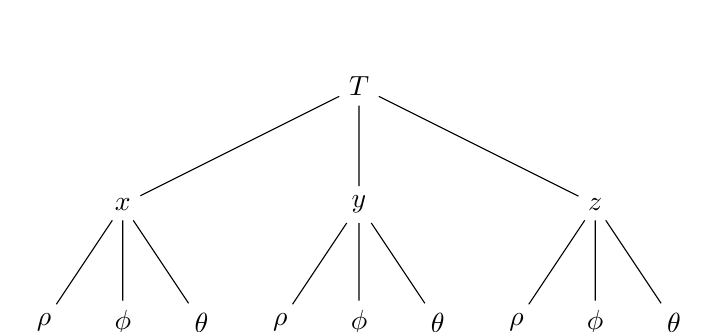
\begin{tikzpicture}[level distance=1.5cm,
          level 1/.style={sibling distance=3cm},
          level 2/.style={sibling distance=1cm}]
          \node {$T$}
            child {node {$x$}
              child {node {$\rho$}}
              child {node {$\phi$}}
              child {node {$\theta$}}
            }
            child {node {$y$}
              child {node {$\rho$}}
              child {node {$\phi$}}
              child {node {$\theta$}}
            }
            child {node {$z$}
              child {node {$\rho$}}
              child {node {$\phi$}}
              child {node {$\theta$}}
            };
        \end{tikzpicture}
        \end{center}
        (In case you're curious, I generated this tree diagram using the very good TikZ library ``trees''. I can share the LaTeX source if you're interested.)
        \end{red}
        
        
        \item[b.] Apply the chain rule to find the partial derivatives $\dfrac{\partial T}{\partial\rho}$, $\dfrac{\partial T}{\partial\phi}$, and $\dfrac{\partial T}{\partial\theta}$.
        
        \begin{red}
        We'll just read the chain rule off the tree:
        \begin{align*}
            \dfrac{\partial T}{\partial\rho} &= 
            \dfrac{\partial T}{\partial x}\cdot
            \dfrac{\partial x}{\partial\rho}
            + 
            \dfrac{\partial T}{\partial y}\cdot
            \dfrac{\partial y}{\partial\rho}
            + 
            \dfrac{\partial T}{\partial z}\cdot
            \dfrac{\partial z}{\partial\rho} \\
            &= 2x\cdot(\sin\phi\cos\theta) 
            + 2y\cdot(\sin\phi\sin\theta)
            -2\cdot(\cos\phi) \\
            &= 2(\rho\sin\phi\cos\theta)\cdot(\sin\phi\cos\theta) 
            + 2(\rho\sin\phi\sin\theta)\cdot(\sin\phi\sin\theta)
            -2\cdot(\cos\phi) \\
            &= 2\rho\sin^2\phi\cos^2\theta + 2\rho\sin^2\phi\sin^2\theta - 2\cos\phi \\
            &= 2\rho\sin^2\phi(\cos^2\theta+\sin^2\theta) - 2\cos\phi \\
            &= 2\rho\sin^2\phi-2\cos\phi
            \\
            \dfrac{\partial T}{\partial\phi} &= 
            \dfrac{\partial T}{\partial x}\cdot
            \dfrac{\partial x}{\partial\phi}
            + 
            \dfrac{\partial T}{\partial y}\cdot
            \dfrac{\partial y}{\partial\phi}
            + 
            \dfrac{\partial T}{\partial z}\cdot
            \dfrac{\partial z}{\partial\phi} \\
            &= 2x\cdot(\rho\cos\phi\cos\theta)
            + 2y\cdot(\rho\cos\phi\sin\theta)
            -2  \cdot(-\rho\sin\phi) \\
            &= 2(\rho\sin\phi\cos\theta)\cdot(\rho\cos\phi\cos\theta)
            + 2(\rho\sin\phi\sin\theta)\cdot(\rho\cos\phi\sin\theta)
            +2  \rho\sin\phi \\
            &= 2\rho^2\sin\phi\cos\phi \cdot (\cos^2\theta + \sin^2 \theta) + 2\rho\sin\phi \\
            &= 2\rho^2\sin\phi\cos\phi + 2\rho\sin\phi
            \\
            \dfrac{\partial T}{\partial\theta} &= 
            \dfrac{\partial T}{\partial x}\cdot
            \dfrac{\partial x}{\partial\theta}
            + 
            \dfrac{\partial T}{\partial y}\cdot
            \dfrac{\partial y}{\partial\theta}
            + 
            \dfrac{\partial T}{\partial z}\cdot
            \dfrac{\partial z}{\partial\theta} \\
            &= 2x\cdot(\rho\sin\phi(-\sin\theta)) 
            + 2y\cdot(\rho\sin\phi\cos\theta)
            -2 \cdot (0) \\
            &= -2(\rho\sin\phi\cos\theta)\cdot(\rho\sin\phi\sin\theta) 
            +2(\rho\sin\phi\sin\theta)\cdot(\rho\sin\phi\cos\theta) \\
            &= -2\rho^2\sin^2\phi\cos\theta\sin\theta + 2\rho^2\sin^2\phi\sin\theta\cos\theta = 0
        \end{align*}
        \end{red}
    \end{enumerate}
\end{enumerate}

\begin{red}
\textbf{Learning Targets Reflection:} Maybe S1, maybe S2, D5, D6.
\end{red}

\end{document}